\chapter{Abstraction}\label{C:abstraction}

% potential examples of abstraction?
% recipies
% programming?
% ???

What do I mean by abstraction?
Capturing the 'essence' of the problem. Without unimportant details.

Related. Representation learning.

What is it?
- Single elements are more complex, but tailored to specific tasks?!
- An idealisation, that ignores unimportant details.
-

Throw away the unimportant details. But how do you know which ones are unimportant?
Example.

Why do we care?

By throwing away details, we can compute more efficiently, less data.
We can learn more efficiently (less noise).
Throwing away unimportant factors of variation will reduce the variance of our
observations and thus allow quicker learning (ref).

- How can we find an abstraction?
- How can we exploit an abstraction?


Toy examples?

- ?
- ?
- ?

History.

- Mathematics, category theory
- Physics?
- Comp sci, programming languages



\begin{itemize}
\tightlist
\item
  exploration, Learning latent state representation for speeding up exploration \cite{Vezzani2019}
\item
  optimal control,
\item
  ???,
\end{itemize}

\begin{displayquote}
\textit{How can an abstraction be used to find an optimal policy?}
\end{displayquote}
insert picture of up down etc.

The three steps of abstraction - transform to a new domain
- solve - apply solution back in original domain.


\begin{displayquote}
The challenge in the single-task case is overcoming the additional cost of discovering the options; this results in a narrow opportunity for performance improvements, but a well-defined objective. In the skill transfer case, the key challenge is predicting the usefulness of a particular option to future tasks, given limited data. \cite{Konidaris2019}
\end{displayquote}

\section{Abstractions for RL}

% types of abstraction we will consider
There are a few different types of abstraction that can be considered for RL:
state abstractions \cite{Littman2006,Haarnoja,Cuccu2018,Zhonga,Vezzani2019,Abel2018,Duan2018,Abel2017,Silver2016a},
action abstractions \cite{Chandak2019,Bester2019,Tennenholtz2019}, temporal abstractions \cite{Rafati,Mankowitz2018,Harutyunyan2017,Fruit2017,Riemer2018,Bacon2018,Achiam2018,Pham2019,Konidaris2018,Haarnoja,Sutton1999,Fruit2017a,Bacon2016a,Jinnai2018,Nachum2018}.
Where there are a couple of main goals of these abstractions; efficient exploration
(\href{https://en.wikipedia.org/wiki/Sample_complexity}{sample complexity})
and / or efficient optimisation (\href{https://en.wikipedia.org/wiki/Computational_complexity_theory}{computational complexity}).

%  but. how can we analyse them?
% tools we can use to analyse an abstraction
Let's say we have a state abstraction, a road is a road: no real difference
between them; gravel, winding, motorway, cliffs-on-either-side...
One of the first things we want to know about the abstraction is:
is it possible for me to act optimally (with respect to some value function)
using this abstraction? If not, what's the damage? In this case, driving 100kph on every road --
because they are all pretty-much-the-same -- might lead to some suboptimal results.
Or, in other words, we want to whether the optimal policy can be approximately represented within an abstracted MDP.

% formal
This notion of suboptimality can be formalised as the representation error of the optimal
policy. Given an abstraction, we want to know how well
the abstraction can represent the optimal policy. \cite{Littman2006, Abel2017}

\begin{align}
\forall_{s\in S, a\in A} \mid Q^{\pi^* }(s, a) - Q^{\pi_{A}^* }(s, a) \mid \le \epsilon
\end{align}

Where $\pi^{* }$ is the optimal policy, and $\pi_{A}^{* }$ is the optimal
policy found using the abstraction.

\subsection{Classes of abstraction for RL}

% \begin{displayquote}
% \textit{But how might we contruct $Q^{\pi_{A}^* }$?}
% \end{displayquote}
%
% There are many different forms an abstraction might take, and ???

\begin{displayquote}
\textit{Given an abstraction, how might a learner use it?}
\end{displayquote}

The abstracted $Q$-function and policy might be constructed on spaces $X, Y$,
$Q_A: X \times Y \to \mathbb R$, $\pi_A: X \to \Delta(Y)$. We can now construct
different classes of learners by giving them access to different types of abstraction.

\begin{align*}
&\phi: S \to X, Y = A \\
&\pi(\phi(s)),\quad Q(\phi(s), a) \tag{State abstraction} \\
&\psi: A\to Y, X = S\\
&\psi^{-1}(\pi(s)),\quad Q(s, \psi(a)) \tag{Action abstraction} \\
&\phi, \psi\\
&\psi^{-1}(\pi(\phi(s))),\quad Q(\phi(s), \psi(a)) \tag{State and action abstraction} \\
&\varphi: S \times A \to Z \\
&\mathop{\text{argmax}}_a V(\varphi(s, a)),\quad V(\varphi(s, a)) \tag{State-action abstraction} \\
\end{align*}

As well as other classes of temporal abstraction. But while they are of great
interest, we do not consider them here.

\begin{displayquote}
\textit{Which class of abstraction should we use?}
\end{displayquote}

Possibly, the most interesting question is about the difference in performance between
the \textit{State and action abstraction} and the \textit{State-action abstraction}.

The state-action abstraction is the most powerful because it allows the compression of the most symmetries. (want to
prove!) And this is part of the motivation behind the successor features \cite{Barreto2017,Dayan1993}.
% The abstraction is able to capture patterns in ??? something about the effects of the actions. Temporal difference models

\subsection{Discovery}

% Why is this hard? How hard is it? Existing work? What is the problem?

\subsubsection{Building an abstraction}

When building an abstraction, you need some notion of how two objects can be similar. (need a ref for this?!)
In RL there are a few possible notions of similarity.

What could be similar? Two states, two actions, two state-actions. Why?
Because they result in the same future rewards? The same future transitions? The same future actions?
Because they can reach the same set of states.

% Two MDPs might be similar?

What about $(s, a, r, s, a)$s? Two $(s, a, r, s, a)$s are similar if?

\begin{enumerate}
\tightlist
\item
  The policy function:
  \(\forall_{\cdot_a, \cdot_b \in D^{* }} \mid \pi(\cdot_a) - \pi(\cdot_b) \mid \le \epsilon\)
  is approximately the same.
\item
  The transition function:
  \(\forall_{\cdot_a, \cdot_b \in D} \mid \tau(\cdot_a) - \tau(\cdot_b)\mid \le \epsilon\)
  is approximately the same.
\item
  The reward function:
  \(\forall_{\cdot_a, \cdot_b \in D} \mid r(\cdot_a) - r(\cdot_b) \mid \le \epsilon\)
  is approximately the same.
\end{enumerate}

A note on the notation used.

Also,

\begin{enumerate}
\def\labelenumi{\arabic{enumi}.}
\setcounter{enumi}{3}
\tightlist
\item
  The policy trajectory:
  \(\forall_{\cdot_a, \cdot_b \in D} \mid \sum_{t=0}^T \parallel \pi(\cdot_a) - \pi(\cdot_b)\parallel_1 \mid \le \epsilon\)
  is approximately the same.
\item
  The transition trajectory:
  \(\forall_{\cdot_a, \cdot_b \in D} \mid \sum_{t=0}^T\parallel \tau(\cdot_{a_t}) - \tau(\cdot_{b_t})\parallel_1\mid \le \epsilon\)
  is approximately the same.
\item
  The reward trajectory:
  \(\forall_{\cdot_a, \cdot_b \in D} \mid \sum_{t=0}^T \parallel r(\cdot_{a_t}) - r(\cdot_{b_t})\parallel_1 \mid \le \epsilon\)
  is approximately the same.
\end{enumerate}

GVFs


\begin{enumerate}
\def\labelenumi{\arabic{enumi}.}
\setcounter{enumi}{6}
\tightlist
\item
  The discounted future policy:
  \(\forall_{\cdot_a, \cdot_b \in D} \mid \Pi(\cdot_a) - \Pi(\cdot_b)\mid \le \epsilon\)
  is approximately the same.
\item
  The discounted future transition:
  \(\forall_{\cdot_a, \cdot_b \in D} \mid \Upsilon(\cdot_a) - \Upsilon (\cdot_b)\mid \le \epsilon\)
  is approximately the same.
\item
  The discounted future reward:
  \(\forall_{\cdot_a, \cdot_b \in D} \mid Q(\cdot_a) - Q(\cdot_b)\mid \le \epsilon\)
  is approximately the same.
\end{enumerate}

For all $\pi \in \Pi$, or just or $\pi^{* }$?

Including any combination of these.
Do some of these make sense?
- Discounted future policy? What is this?
- How is the future policy different from the future trajectory?
- ?

\textbf{Q:} Which is best?

\begin{quote}
\textbf{Claim 1:} 9.(the value fn) will yield the most compression,
while performing well. But, it is a task specific representation, thus
it will not transfer / generalise well.
\end{quote}


\cite{Littman2006} give 5 classes of state abstraction, and show that ...???
Here is a further generalisation


$V(s) - V(s')$ as a similarity measure tells us very little. Because...?



\subsection{Examples}

\subsubsection{State abstraction}

State abstraction groups together states that are similar. For example,
sprinting 100m is equivalent regardless of which track lane you are in.

\subsubsection{Action abstraction}

Action abstraction groups together actions that are similar. For
example, X and Y both yeild the state change in state, \textgreater{}
Approximation perspective: we have a set of options and we want to use
them to approximate the optimal policy. A good set of options can
efficiently achieve an accurate approximation.

\subsubsection{State-action abstraction}

\emph{(Some intuition behind claim 2.)}

Imagine you are in a mirror symmetric maze. It should not matter to you
which side of mirror you are on.

\begin{figure}
\centering
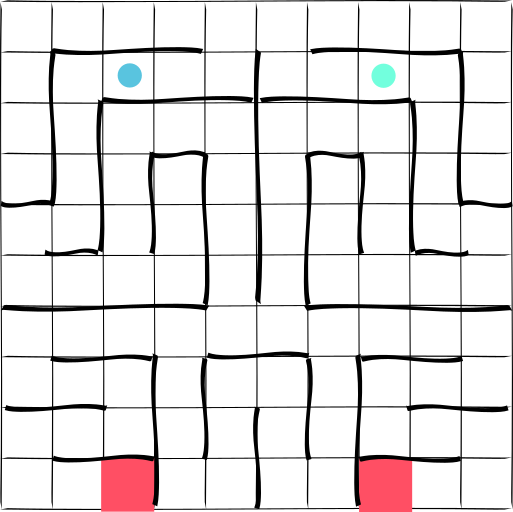
\includegraphics[width=0.5\textwidth,height=0.5\textheight]{../../pictures/drawings/maze.png}
\caption{maze.png}
\end{figure}

This reduces the state-action space by half!
\(\frac{1}{2}\mid S \mid \times \mid A \mid\). Note: just using state
abstraction it is not possible to achieve this reduction. Mirrored
states are not equivalent as the actions are inverted.

While other learners can still solve this problem. They miss out on
efficiency gains by abstracting first.

This intuition leads to our work in section ... (symetric abstractions).

\subsubsection{Temporal abstraction}

???


\subsection{Discussion}

A main issue with this framework for analysing abstraction is that it does not consider
the sample or computational complexity of finding the optimal policy. Only that, under the abstraction,
it exists.

Also, we have not discussed the discovery of / how to construct the abstraction.

\begin{center}\rule{0.5\linewidth}{\linethickness}\end{center}

Want a general way (a function) to take an abstraction of an MDP
(defined by certain propreties) and return the difference between its
optimal policy and the true optimal policy. Want automated computational
complexity to solve this! Actually, we are not considering computational
complexity here only approximation error. For that can we just use
automatic differentiation!? Want a way to get bounds for all of these
combinations!

Requires the evaluation of expensive integrals?!?
